% Figure 5: Power Density vs Frequency
% Author: Dr. Computernonymouse
% Description: Log-log plot showing extractable power density as function of
%              operating frequency for different efficiency scenarios

\documentclass[tikz,border=10pt]{standalone}
\usepackage{pgfplots}
\usepackage{amsmath}
\usepackage{amssymb}
\usepackage{siunitx}

\pgfplotsset{compat=1.18}
\usetikzlibrary{arrows.meta,patterns}

% Define colors for different curves
\definecolor{theoretical}{RGB}{214,39,40}
\definecolor{coupled}{RGB}{255,127,14}
\definecolor{realistic}{RGB}{31,119,180}
\definecolor{operating}{RGB}{44,160,44}
\definecolor{gridcolor}{RGB}{128,128,128}

% PGFPlots settings for scientific notation
\pgfplotsset{
    /pgfplots/log base 10 number format code/.code={
        $10^{\pgfmathprintnumber{#1}}$
    }
}

\begin{document}

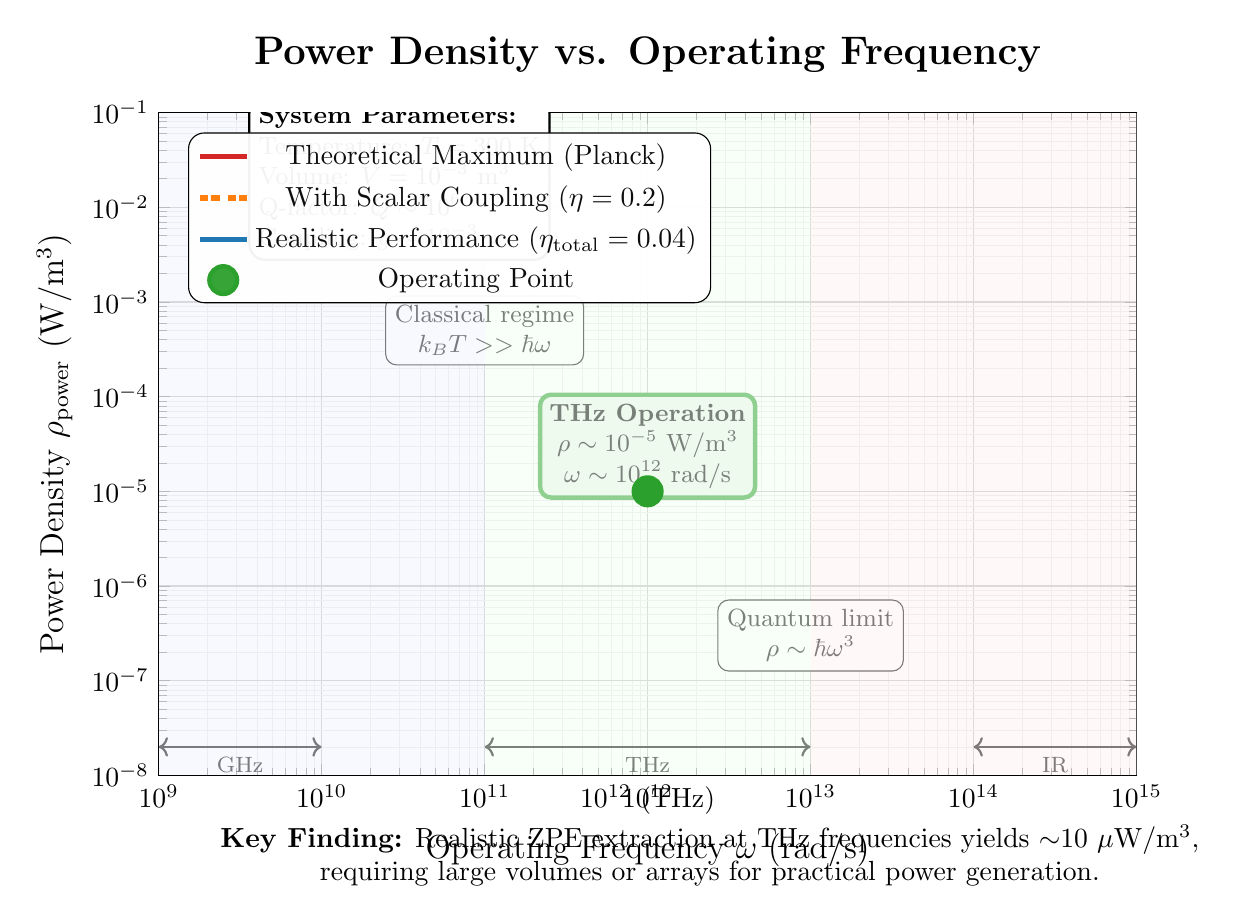
\begin{tikzpicture}

\begin{loglogaxis}[
    width=14cm,
    height=10cm,
    xlabel={Operating Frequency $\omega$ (rad/s)},
    ylabel={Power Density $\rho_{\text{power}}$ (W/m$^3$)},
    xmin=1e9, xmax=1e15,
    ymin=1e-8, ymax=1e-1,
    grid=both,
    minor tick num=9,
    major grid style={line width=0.5pt,draw=gridcolor!50},
    minor grid style={line width=0.2pt,draw=gridcolor!20},
    xlabel style={font=\large},
    ylabel style={font=\large},
    tick label style={font=\normalsize},
    legend pos=north west,
    legend style={
        font=\normalsize,
        fill=white,
        fill opacity=0.95,
        draw=black,
        rounded corners=2mm,
        row sep=2pt
    },
    log basis x={10},
    log basis y={10},
    extra x ticks={1e12},
    extra x tick labels={$10^{12}$ (THz)},
    extra x tick style={
        grid=major,
        grid style={line width=1pt,draw=operating!50,dashed}
    },
    title={Power Density vs. Operating Frequency},
    title style={font=\Large\bfseries,yshift=5pt},
    every axis plot/.append style={ultra thick}
]

% Theoretical maximum (Planck distribution approximation)
\addplot[
    theoretical,
    line width=2pt,
    smooth,
    samples=50,
    domain=1e9:1e15
] {1e-15 * x^3 / (exp(1.05e-34 * x / (1.38e-23 * 300)) - 1)};
\addlegendentry{Theoretical Maximum (Planck)}

% With scalar coupling (20% efficiency)
\addplot[
    coupled,
    line width=2pt,
    dashed,
    smooth,
    samples=50,
    domain=1e9:1e15
] {0.2 * 1e-15 * x^3 / (exp(1.05e-34 * x / (1.38e-23 * 300)) - 1)};
\addlegendentry{With Scalar Coupling ($\eta = 0.2$)}

% Realistic performance (4% total efficiency)
\addplot[
    realistic,
    line width=2pt,
    smooth,
    samples=50,
    domain=1e9:1e15
] {0.04 * 1e-15 * x^3 / (exp(1.05e-34 * x / (1.38e-23 * 300)) - 1)};
\addlegendentry{Realistic Performance ($\eta_{\text{total}} = 0.04$)}

% Operating point marker
\addplot[
    operating,
    only marks,
    mark=*,
    mark size=5pt
] coordinates {(1e12, 1e-5)};
\addlegendentry{Operating Point}

% Annotations
\node[align=center,font=\small,draw=black,rounded corners,fill=white!90]
    at (axis cs:1e13,3e-7) {
        Quantum limit\\
        $\rho \sim \hbar\omega^3$
    };

\node[align=center,font=\small,draw=black,rounded corners,fill=white!90]
    at (axis cs:1e11,5e-4) {
        Classical regime\\
        $k_B T >> \hbar\omega$
    };

\node[align=center,font=\small,draw=operating,ultra thick,rounded corners,fill=operating!10]
    at (axis cs:1e12,3e-5) {
        \textbf{THz Operation}\\
        $\rho \sim 10^{-5}$ W/m$^3$\\
        $\omega \sim 10^{12}$ rad/s
    };

% Frequency bands
\draw[<->,thick] (axis cs:1e9,2e-8) -- (axis cs:1e10,2e-8)
    node[midway,below,font=\footnotesize] {GHz};
\draw[<->,thick] (axis cs:1e11,2e-8) -- (axis cs:1e13,2e-8)
    node[midway,below,font=\footnotesize] {THz};
\draw[<->,thick] (axis cs:1e14,2e-8) -- (axis cs:1e15,2e-8)
    node[midway,below,font=\footnotesize] {IR};

% Shaded regions for different regimes
\fill[blue!5,opacity=0.5] (axis cs:1e9,1e-8) rectangle (axis cs:1e11,1e-1);
\fill[green!5,opacity=0.5] (axis cs:1e11,1e-8) rectangle (axis cs:1e13,1e-1);
\fill[red!5,opacity=0.5] (axis cs:1e13,1e-8) rectangle (axis cs:1e15,1e-1);

% Technical parameters box
\node[draw=black,thick,rounded corners=2mm,fill=white!95,
      align=left,font=\small] at (axis cs:3e10,2e-2) {
    \textbf{System Parameters:}\\
    Temperature: $T = 300$ K\\
    Volume: $V = 10^{-3}$ m$^3$\\
    Q-factor: $Q \sim 10^6$\\
    Coupling: $g \sim 10^{-3}$
};

\end{loglogaxis}

% Additional information below plot
\node[below,font=\normalsize,align=center] at (7,-0.5) {
    \textbf{Key Finding:} Realistic ZPE extraction at THz frequencies yields $\sim$10 $\mu$W/m$^3$,\\
    requiring large volumes or arrays for practical power generation.
};

\end{tikzpicture}

\end{document}